% !TEX program = xelatex
\RequirePackage{fontspec}
\DeclareFontFamily{TU}{ptm}{}
\DeclareFontShape{TU}{ptm}{m}{n}{<->"[lmroman10-regular.otf]"}{}
\DeclareFontShape{TU}{ptm}{bx}{n}{<->"[lmroman10-bold.otf]"}{}
\DeclareFontShape{TU}{ptm}{m}{it}{<->"[lmroman10-italic.otf]"}{}
\DeclareFontShape{TU}{ptm}{bx}{it}{<->"[lmroman10-bolditalic.otf]"}{}
\documentclass[conference,a4paper]{IEEEtran}
\setmainfont[Path=fonts/,BoldFont=texgyretermes-bold.otf,ItalicFont=texgyretermes-italic.otf,BoldItalicFont=texgyretermes-bolditalic.otf]{texgyretermes-regular.otf}
\newfontfamily\japanesefont[Path=fonts/]{NotoSerifCJKjp-Regular.otf}
\usepackage{cite}
\usepackage{amsmath,amssymb}
\usepackage{array}
\usepackage{graphicx}
\usepackage{textcomp}
\usepackage{tikz}
\usetikzlibrary{arrows.meta,positioning}
\usepackage{url}
% Compact float spacing; retain the IEEE text size and page geometry.
\setlength{\textfloatsep}{9pt plus 2pt minus 2pt}
\setlength{\dbltextfloatsep}{9pt plus 2pt minus 2pt}
\setlength{\floatsep}{7pt plus 2pt minus 2pt}
\setlength{\dblfloatsep}{7pt plus 2pt minus 2pt}
\begin{document}
\title{Evaluating Pedigree Graph Features Beyond Recent Form and Market Information in Horse Racing}
\author{}
\maketitle

\begin{abstract}
This study asks whether a pedigree-graph feature group improves top-three prediction beyond recent history when an ancestor-based representation is constructed consistently across chronological splits. We compare context and history, the original direct-else-ancestor graph pipeline, an ancestor-rule graph pipeline and a supervised chronological parent-performance control on Japan Racing Association flat races. The observed 2010--2025 cohort has 725,999 entries in 51,313 races. Across three classifier families and two surfaces, all six turf average-precision contrasts of the ancestor-rule pipeline against history or the parent control are negative with descriptive paired intervals below zero; the six dirt intervals include zero. All 12 primary Hit@3 intervals include zero. A secondary CatBoost dirt comparison favors the ancestor-rule pipeline over the original mixed pipeline, but does not isolate a fallback effect. These comparisons are exploratory because the test cohort was previously examined. The same construction rule does not equalize coverage or eliminate the original graph's historical-topology limitations. A separate historical analysis retains final-market comparisons, which are retrospective and are not controls in the new four-arm study.
\end{abstract}
\begin{IEEEkeywords}
graph embedding, horse racing, Node2Vec, pedigree, predictive modeling
\end{IEEEkeywords}

\section{Introduction}
For a top-three prediction system, a pedigree representation is useful to the extent that it improves prediction beyond information already available from recent performance. Assessing that increment is difficult when training horses have direct graph vectors but many later entrants do not. A fallback based on embedded ancestors then changes the representation used for those entrants. Applying one construction rule across splits addresses that difference in procedure, although it does not make coverage or feature distributions identical.

We examine Japan Racing Association (JRA) flat races using a fixed training-root pedigree graph and chronological partitions \cite{jraResults,netkeibaRace,netkeibaDb,grover2016}. The central question is whether the specified graph-feature pipeline adds predictive value beyond race context and recent history when ancestor-based construction is used throughout, and how it compares with a simple parent-performance control. Four pipelines use the same cohort, three classifier families and separate turf and dirt models. The two primary comparisons are the ancestor-rule graph against history and against the parent control; the comparison with the original direct-else-ancestor pipeline is secondary. The test cohort had already been examined before this design was fixed, so these comparisons are post-test exploratory. The study evaluates particular feature pipelines rather than a new graph architecture or a causal effect of ancestry. We retain the earlier retrospective market analysis as separate context; the new four-arm study contains no market predictors.

\section{Related Work}
Sugiura \cite{sugiura2026} studied temporally held-out JRA win and place-rule outcomes using recent history, sire and damsire information and matched feature-block comparisons, without final odds or popularity. The place-rule label is not identical to the fixed top-three outcome here. A 2024 Japanese technical report proposes a pedigree graph neural network for future racehorse performance \cite{oikawa2024}; its detailed target and controls could not be established from the accessible abstract. Gulum \cite{gulum2018} used graph-derived features for paired-horse prediction. Oda and Onogi \cite{oda2024} studied pedigree-based breeding values for adjusted velocity and graded-winner status, different prediction targets from ours. Chung \emph{et al.} \cite{chung2024} considered race ranking in Seoul; we rank entry-classifier scores and do not evaluate a dedicated ranking model. Earlier racing studies also motivate history and market controls \cite{silverman2013,pudaruth2013}, while pedigree research motivates, but does not establish, incremental predictive value \cite{bailey2022}.

Our bounded contribution is the same-cohort evaluation of a fixed ancestor-rule graph pipeline against history and a specified chronological parent-outcome comparator, with the original mixed-representation pipeline as a secondary reference. Temporal validation, feature-block comparisons, race bootstrap and pedigree graphs each have prior precedents; none is claimed as a new method here.

\section{Methods}
\subsection{Cohort and Prediction Task}
We use the original observed JRA flat-race cohort, with race results and pedigree records collected through Netkeiba \cite{netkeibaRace,netkeibaDb}. Eligible entries are divided by race date into 2010--2021 training, 2022--2023 validation and 2024--2025 test partitions, retaining complete race rosters (Table~\ref{tab:cohort}). The observed collection is not the entire JRA racing universe \cite{jraStats2yo,jraStats3up}. The binary label indicates an official top-three finish; documented non-finishers are negative, pre-start withdrawals are excluded, and all horses sharing a top-three position in a dead heat are positive. Models are fitted separately for turf and dirt. The test races had been inspected in earlier analyses, making this study exploratory rather than a fresh confirmatory test.

\begin{table}[!t]
\caption{Chronological Cohort and Test Surface Denominators}
\label{tab:cohort}
\centering
\begin{tabular}{lrrr}
\hline
Partition & Years & Races & Entries \\
\hline
Training & 2010--2021 & 38,447 & 548,756 \\
Validation & 2022--2023 & 6,401 & 88,106 \\
Test, turf & 2024--2025 & 3,246 & 43,477 \\
Test, dirt & 2024--2025 & 3,219 & 45,660 \\
\hline
Total & 2010--2025 & 51,313 & 725,999 \\
\hline
\end{tabular}
\end{table}


All four arms use the same 43 race-context and recent-history predictors: 12 context variables, an observed-start count, three history-availability indicators and nine attributes for each of up to three previous starts. History uses eligible observed starts strictly before the target date, including observed jump starts, although targets are flat races. Missing history remains missing. Final odds and popularity are not predictors in these four arms. Category maps are fitted on each training surface, distinguishing missing, unseen and categories occurring fewer than five times; classifiers use native categorical handling and numeric missing values.

\subsection{Graph and Feature Pipelines}
The original three-generation graph is the union of pedigrees rooted at training-period starters, with 62,270 roots, 93,474 nodes and 173,412 edges. Parent--child edges are projected to an undirected graph for Node2Vec \cite{grover2016}. The fixed configuration uses 64 dimensions, 10 walks per node, walk length 80, window 5, five epochs, $p=1$ and $q=0.5$. Each seed has its own fixed vectors and 64 cluster centroids. Within a seed, both graph arms use the same original vector space and centroids. The graph is not reconstructed for each target date or held-out horse. It includes relationships contributed by later training roots, and the focal horse may have influenced graph topology even when its own vector is not directly used. Pedigree records were collected retrospectively, and their availability at each historical cutoff was not verified.

The four feature pipelines are H (context and history); $G_{\mathrm{mixed}}$ (H plus the original graph group, using the focal vector when available and otherwise an ancestor vector); $G_{\mathrm{ancestor}}$ (the same graph group and frozen space, applying the ancestor rule to every entry); and P (H plus nine chronological parent-performance features). The graph group comprises 64 vector coordinates and five descriptors: representation status, selected depth, number of available ancestors, missingness and nearest-centroid category. For the ancestor rule, parents, grandparents and great-grandparents are examined in order. At the first generation containing embedded ancestors, their unique vectors are averaged equally. $G_{\mathrm{ancestor}}$ excludes a focal identifier encountered through a cycle; $G_{\mathrm{mixed}}$ retains the original fallback implementation. If no ancestor is available, the vector is zero with an explicit missing status and cluster. Otherwise the closest frozen centroid is assigned by squared Euclidean distance, with lowest index resolving an exact tie. Table~\ref{tab:focused_coverage} reports coverage. The same $G_{\mathrm{ancestor}}$ rule is used across partitions, but coverage, depth and vector distributions can still differ. The two graph arms compare complete pipelines, not an isolated intervention on fallback.

\begin{table*}[!t]
\caption{Graph Representation Coverage by Partition and Surface}
\label{tab:focused_coverage}
\centering
\begin{tabular}{llrrrrrr}
\hline
& & & $G_{\mathrm{mixed}}$ & \multicolumn{3}{c}{$G_{\mathrm{ancestor}}$: first available depth} & Missing \\
Partition & Surface & Entries & direct & 1 & 2 & 3 & (either) \\
\hline
Training & Turf & 271,549 & 271,549 & 271,549 & 0 & 0 & 0 \\
Training & Dirt & 277,207 & 277,207 & 277,207 & 0 & 0 & 0 \\
Validation & Turf & 42,783 & 21,708 & 42,580 & 202 & 1 & 0 \\
Validation & Dirt & 45,323 & 24,398 & 45,081 & 242 & 0 & 0 \\
Test & Turf & 43,477 & 5,641 & 42,866 & 596 & 15 & 0 \\
Test & Dirt & 45,660 & 5,506 & 44,613 & 1,039 & 8 & 0 \\
\hline
\end{tabular}
\par\smallskip Counts are entries, not distinct horses; counts are identical across graph seeds. $G_{\mathrm{mixed}}$ uses fallback for entries without direct vectors. All test entries have sire, dam and damsire identifiers. Their P zero-prior counts are 13,103/17,941/1,982 on turf and 13,182/20,027/2,371 on dirt, in that order.
\end{table*}


\subsection{Chronological Parent Control}
P adds, for sire, dam and damsire separately, an identifier-availability indicator, a count of eligible prior same-surface starts and a smoothed top-three rate. The count and successes exclude all starts of the focal horse and include only training outcomes strictly earlier than the target date; same-day outcomes are unavailable to each other. For a count $n$ and positive count $s$, the fixed rate is $(s+20\times0.20)/(n+20)$. An absent identifier and a known identifier with no qualifying starts both have count zero and rate 0.20, distinguished by the availability indicator. These are supervised outcome-derived summaries, not genetic-effect estimates; the constant prior is a prespecified regularizer rather than an estimated population rate.

Training summaries expand by date, while the map is frozen at the end of 2021 for all validation and test entries, with focal-horse contributions removed. It never incorporates validation or test outcomes. The source history starts in 2010, so earlier parent performance is left-censored; the frozen map also becomes older relative to later targets. The categorical preprocessing setting that disables external target encoding does not remove P's supervised parent summaries.

\subsection{Historical Market Comparison}
The original analysis on the same cohort is retained separately. A uses context and history; B adds categorical sire/dam identifiers; C adds the original graph group; D adds retrospectively recorded final odds and popularity to A; E adds those market fields to C; and F uses final odds alone. The historical comparisons C--A, C--B, E--D and E--C use independently tuned pipelines. Seven of 60 selected historical tuning curves reached the cap, with best rounds potentially earlier. Final odds and popularity enter together and their individual contributions cannot be separated. The four new arms do not include market fields and do not test $G_{\mathrm{ancestor}}$ or P beyond market information. Final-field, going, weight and market timestamps were not verified at a common pre-start horizon.

\subsection{Fitting and Evaluation}
XGBoost, LightGBM and CatBoost \cite{chen2016,ke2017,prokhorenkova2018} are tuned independently for each arm, family and surface. Four fixed candidates are fitted with seed 0, a maximum of 1,200 rounds and early-stopping patience of 75. Candidate selection uses validation average precision (AP); candidates within $10^{-6}$ of the highest AP are ordered by higher validation Hit@3, fewer best rounds and then candidate identifier. The selected parameters and best-round count are refitted using the training partition alone for seeds 0, 1 and 2; validation is not added to the final fit. Of 96 candidate tuning curves, 21 reached the cap; four of 24 selected curves reached it, while no selected best round or refit round was 1,200. A capped curve can have an earlier best round. Equal budgets do not establish equally adequate tuning. Graph and classifier seeds are paired, so their sources of variation are not separately identified.

The primary score is entry-level AP \cite{saito2015}, which aggregates entries with equal scores at the same threshold. The secondary score, race-mean Hit@3, is the fraction of the three highest-scored entries in each full race that finished in the top three, averaged across races. For this within-race selection only, score ties are ordered by horse number and then horse identifier. We average seed-specific scores and paired differences, not predictions. The primary contrasts are $G_{\mathrm{ancestor}}$--H and $G_{\mathrm{ancestor}}$--P; $G_{\mathrm{ancestor}}$--$G_{\mathrm{mixed}}$ is secondary. All are reported by family and surface for both scores.

For each surface, the same 2,000 whole-race bootstrap draws are used across arms, families and seeds. Each draw resamples complete races with replacement, retains repeated draws, recomputes each seed's score, and averages the paired differences across seeds. The 2.5th and 97.5th percentiles give descriptive paired 95\% intervals conditional on the fitted models. They do not include retraining uncertainty, adjust for multiple comparisons or restore confirmatory inference after prior test examination; repeated horses also create dependence beyond races. An interval containing zero does not establish equivalence.

\section{Results and Discussion}
\subsection{Four-Arm Comparison}
Table~\ref{tab:focused_scores} gives both scores and seed dispersion for every arm, family and surface. Fig.~\ref{fig:focused_contrasts} shows all primary and secondary AP contrasts; the companion retains all 36 AP and Hit@3 contrast intervals and all 72 seed-level score rows. The estimates are exploratory comparisons of independently tuned feature pipelines on a previously examined test set.

\begin{table*}[!t]
\caption{Four-arm test scores across the three fitted seeds}
\label{tab:focused_scores}
\centering
\begin{tabular}{lllcc}
\hline
Surface & Family & Arm & AP & Hit@3 \\
\hline
Turf & XGBoost & H & 0.4710 $\pm$ 0.0006 & 0.4580 $\pm$ 0.0004 \\
Turf & XGBoost & $G_{\mathrm{mixed}}$ & 0.4631 $\pm$ 0.0010 & 0.4600 $\pm$ 0.0007 \\
Turf & XGBoost & $G_{\mathrm{ancestor}}$ & 0.4621 $\pm$ 0.0002 & 0.4603 $\pm$ 0.0019 \\
Turf & XGBoost & P & 0.4705 $\pm$ 0.0002 & 0.4621 $\pm$ 0.0015 \\
Turf & LightGBM & H & 0.4738 $\pm$ 0.0005 & 0.4585 $\pm$ 0.0010 \\
Turf & LightGBM & $G_{\mathrm{mixed}}$ & 0.4663 $\pm$ 0.0004 & 0.4645 $\pm$ 0.0006 \\
Turf & LightGBM & $G_{\mathrm{ancestor}}$ & 0.4664 $\pm$ 0.0010 & 0.4629 $\pm$ 0.0015 \\
Turf & LightGBM & P & 0.4736 $\pm$ 0.0002 & 0.4646 $\pm$ 0.0021 \\
Turf & CatBoost & H & 0.4725 $\pm$ 0.0005 & 0.4601 $\pm$ 0.0005 \\
Turf & CatBoost & $G_{\mathrm{mixed}}$ & 0.4668 $\pm$ 0.0002 & 0.4627 $\pm$ 0.0011 \\
Turf & CatBoost & $G_{\mathrm{ancestor}}$ & 0.4667 $\pm$ 0.0006 & 0.4638 $\pm$ 0.0042 \\
Turf & CatBoost & P & 0.4712 $\pm$ 0.0001 & 0.4627 $\pm$ 0.0016 \\
Dirt & XGBoost & H & 0.4561 $\pm$ 0.0007 & 0.4634 $\pm$ 0.0012 \\
Dirt & XGBoost & $G_{\mathrm{mixed}}$ & 0.4541 $\pm$ 0.0009 & 0.4616 $\pm$ 0.0008 \\
Dirt & XGBoost & $G_{\mathrm{ancestor}}$ & 0.4552 $\pm$ 0.0007 & 0.4634 $\pm$ 0.0013 \\
Dirt & XGBoost & P & 0.4575 $\pm$ 0.0009 & 0.4654 $\pm$ 0.0020 \\
Dirt & LightGBM & H & 0.4585 $\pm$ 0.0006 & 0.4650 $\pm$ 0.0013 \\
Dirt & LightGBM & $G_{\mathrm{mixed}}$ & 0.4567 $\pm$ 0.0010 & 0.4614 $\pm$ 0.0020 \\
Dirt & LightGBM & $G_{\mathrm{ancestor}}$ & 0.4578 $\pm$ 0.0004 & 0.4632 $\pm$ 0.0019 \\
Dirt & LightGBM & P & 0.4606 $\pm$ 0.0006 & 0.4680 $\pm$ 0.0023 \\
Dirt & CatBoost & H & 0.4523 $\pm$ 0.0004 & 0.4603 $\pm$ 0.0014 \\
Dirt & CatBoost & $G_{\mathrm{mixed}}$ & 0.4525 $\pm$ 0.0011 & 0.4619 $\pm$ 0.0020 \\
Dirt & CatBoost & $G_{\mathrm{ancestor}}$ & 0.4544 $\pm$ 0.0009 & 0.4644 $\pm$ 0.0011 \\
Dirt & CatBoost & P & 0.4553 $\pm$ 0.0015 & 0.4643 $\pm$ 0.0018 \\
\hline
\end{tabular}
\par\smallskip Scores are fractions, shown as mean $\pm$ sample SD across three paired seeds. The test was previously examined. Cohort denominators are in Table~\ref{tab:cohort}; graph coverage and parent-summary availability are in Table~\ref{tab:focused_coverage}.
\end{table*}

\begin{figure}[!t]
\centering
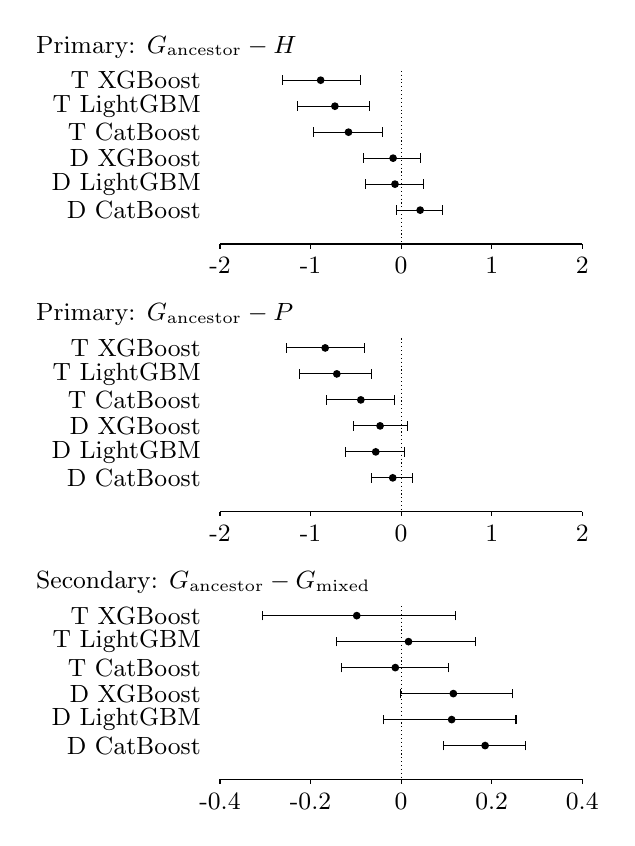
\begin{tikzpicture}[x=1cm,y=1cm]
\small
\node[anchor=west] at (0,-0.000) {Primary: $G_{\mathrm{ancestor}}-H$};
\node[anchor=east] at (2.32,-0.420) {T XGBoost};
\draw (3.2385,-0.420) -- (4.2323,-0.420);
\draw (3.2385,-0.480) -- (3.2385,-0.360);
\draw (4.2323,-0.480) -- (4.2323,-0.360);
\fill (3.7279,-0.420) circle (1.4pt);
\node[anchor=east] at (2.32,-0.750) {T LightGBM};
\draw (3.4320,-0.750) -- (4.3469,-0.750);
\draw (3.4320,-0.810) -- (3.4320,-0.690);
\draw (4.3469,-0.810) -- (4.3469,-0.690);
\fill (3.9088,-0.750) circle (1.4pt);
\node[anchor=east] at (2.32,-1.080) {T CatBoost};
\draw (3.6377,-1.080) -- (4.5131,-1.080);
\draw (3.6377,-1.140) -- (3.6377,-1.020);
\draw (4.5131,-1.140) -- (4.5131,-1.020);
\fill (4.0813,-1.080) circle (1.4pt);
\node[anchor=east] at (2.32,-1.410) {D XGBoost};
\draw (4.2665,-1.410) -- (4.9967,-1.410);
\draw (4.2665,-1.470) -- (4.2665,-1.350);
\draw (4.9967,-1.470) -- (4.9967,-1.350);
\fill (4.6478,-1.410) circle (1.4pt);
\node[anchor=east] at (2.32,-1.740) {D LightGBM};
\draw (4.2961,-1.740) -- (5.0390,-1.740);
\draw (4.2961,-1.800) -- (4.2961,-1.680);
\draw (5.0390,-1.800) -- (5.0390,-1.680);
\fill (4.6719,-1.740) circle (1.4pt);
\node[anchor=east] at (2.32,-2.070) {D CatBoost};
\draw (4.6866,-2.070) -- (5.2736,-2.070);
\draw (4.6866,-2.130) -- (4.6866,-2.010);
\draw (5.2736,-2.130) -- (5.2736,-2.010);
\fill (4.9917,-2.070) circle (1.4pt);
\draw[densely dotted] (4.7500,-0.300) -- (4.7500,-2.500);
\draw (2.45,-2.500) -- (7.05,-2.500);
\draw (2.4500,-2.500) -- (2.4500,-2.560) node[below] {-2};
\draw (3.6000,-2.500) -- (3.6000,-2.560) node[below] {-1};
\draw (4.7500,-2.500) -- (4.7500,-2.560) node[below] {0};
\draw (5.9000,-2.500) -- (5.9000,-2.560) node[below] {1};
\draw (7.0500,-2.500) -- (7.0500,-2.560) node[below] {2};
\node[anchor=west] at (0,-3.400) {Primary: $G_{\mathrm{ancestor}}-P$};
\node[anchor=east] at (2.32,-3.820) {T XGBoost};
\draw (3.2982,-3.820) -- (4.2878,-3.820);
\draw (3.2982,-3.880) -- (3.2982,-3.760);
\draw (4.2878,-3.880) -- (4.2878,-3.760);
\fill (3.7857,-3.820) circle (1.4pt);
\node[anchor=east] at (2.32,-4.150) {T LightGBM};
\draw (3.4620,-4.150) -- (4.3758,-4.150);
\draw (3.4620,-4.210) -- (3.4620,-4.090);
\draw (4.3758,-4.210) -- (4.3758,-4.090);
\fill (3.9330,-4.150) circle (1.4pt);
\node[anchor=east] at (2.32,-4.480) {T CatBoost};
\draw (3.7965,-4.480) -- (4.6691,-4.480);
\draw (3.7965,-4.540) -- (3.7965,-4.420);
\draw (4.6691,-4.540) -- (4.6691,-4.420);
\fill (4.2381,-4.480) circle (1.4pt);
\node[anchor=east] at (2.32,-4.810) {D XGBoost};
\draw (4.1407,-4.810) -- (4.8299,-4.810);
\draw (4.1407,-4.870) -- (4.1407,-4.750);
\draw (4.8299,-4.870) -- (4.8299,-4.750);
\fill (4.4825,-4.810) circle (1.4pt);
\node[anchor=east] at (2.32,-5.140) {D LightGBM};
\draw (4.0443,-5.140) -- (4.7953,-5.140);
\draw (4.0443,-5.200) -- (4.0443,-5.080);
\draw (4.7953,-5.200) -- (4.7953,-5.080);
\fill (4.4275,-5.140) circle (1.4pt);
\node[anchor=east] at (2.32,-5.470) {D CatBoost};
\draw (4.3784,-5.470) -- (4.8995,-5.470);
\draw (4.3784,-5.530) -- (4.3784,-5.410);
\draw (4.8995,-5.530) -- (4.8995,-5.410);
\fill (4.6434,-5.470) circle (1.4pt);
\draw[densely dotted] (4.7500,-3.700) -- (4.7500,-5.900);
\draw (2.45,-5.900) -- (7.05,-5.900);
\draw (2.4500,-5.900) -- (2.4500,-5.960) node[below] {-2};
\draw (3.6000,-5.900) -- (3.6000,-5.960) node[below] {-1};
\draw (4.7500,-5.900) -- (4.7500,-5.960) node[below] {0};
\draw (5.9000,-5.900) -- (5.9000,-5.960) node[below] {1};
\draw (7.0500,-5.900) -- (7.0500,-5.960) node[below] {2};
\node[anchor=west] at (0,-6.800) {Secondary: $G_{\mathrm{ancestor}}-G_{\mathrm{mixed}}$};
\node[anchor=east] at (2.32,-7.220) {T XGBoost};
\draw (2.9845,-7.220) -- (5.4389,-7.220);
\draw (2.9845,-7.280) -- (2.9845,-7.160);
\draw (5.4389,-7.280) -- (5.4389,-7.160);
\fill (4.1863,-7.220) circle (1.4pt);
\node[anchor=east] at (2.32,-7.550) {T LightGBM};
\draw (3.9301,-7.550) -- (5.6971,-7.550);
\draw (3.9301,-7.610) -- (3.9301,-7.490);
\draw (5.6971,-7.610) -- (5.6971,-7.490);
\fill (4.8436,-7.550) circle (1.4pt);
\node[anchor=east] at (2.32,-7.880) {T CatBoost};
\draw (3.9932,-7.880) -- (5.3536,-7.880);
\draw (3.9932,-7.940) -- (3.9932,-7.820);
\draw (5.3536,-7.940) -- (5.3536,-7.820);
\fill (4.6762,-7.880) circle (1.4pt);
\node[anchor=east] at (2.32,-8.210) {D XGBoost};
\draw (4.7390,-8.210) -- (6.1605,-8.210);
\draw (4.7390,-8.270) -- (4.7390,-8.150);
\draw (6.1605,-8.270) -- (6.1605,-8.150);
\fill (5.4131,-8.210) circle (1.4pt);
\node[anchor=east] at (2.32,-8.540) {D LightGBM};
\draw (4.5229,-8.540) -- (6.2089,-8.540);
\draw (4.5229,-8.600) -- (4.5229,-8.480);
\draw (6.2089,-8.600) -- (6.2089,-8.480);
\fill (5.3916,-8.540) circle (1.4pt);
\node[anchor=east] at (2.32,-8.870) {D CatBoost};
\draw (5.2924,-8.870) -- (6.3288,-8.870);
\draw (5.2924,-8.930) -- (5.2924,-8.810);
\draw (6.3288,-8.930) -- (6.3288,-8.810);
\fill (5.8166,-8.870) circle (1.4pt);
\draw[densely dotted] (4.7500,-7.100) -- (4.7500,-9.300);
\draw (2.45,-9.300) -- (7.05,-9.300);
\draw (2.4500,-9.300) -- (2.4500,-9.360) node[below] {-0.4};
\draw (3.6000,-9.300) -- (3.6000,-9.360) node[below] {-0.2};
\draw (4.7500,-9.300) -- (4.7500,-9.360) node[below] {0};
\draw (5.9000,-9.300) -- (5.9000,-9.360) node[below] {0.2};
\draw (7.0500,-9.300) -- (7.0500,-9.360) node[below] {0.4};
\end{tikzpicture}
\caption{All prespecified AP differences, in percentage points (100 times the fraction difference). T and D denote turf and dirt. Points average paired seed-specific differences; whiskers are descriptive 95\% paired whole-race bootstrap percentile intervals, conditional on the fitted models and unadjusted for multiple comparisons. Panels use their indicated scales. The test was previously examined. Denominators and coverage are in Tables~\ref{tab:cohort} and \ref{tab:focused_coverage}.}
\label{fig:focused_contrasts}
\end{figure}


On turf, $G_{\mathrm{ancestor}}$--H AP differences are $-0.0089$, $-0.0073$ and $-0.0058$ for XGBoost, LightGBM and CatBoost; the corresponding $G_{\mathrm{ancestor}}$--P differences are $-0.0084$, $-0.0071$ and $-0.0045$. All six descriptive paired intervals lie below zero. On dirt, all six primary AP intervals include zero. All 12 primary Hit@3 intervals include zero. Thus the tested ancestor-rule graph group does not establish a consistent AP benefit over H or P across families and surfaces; intervals containing zero do not establish equivalence.

The secondary $G_{\mathrm{ancestor}}$--$G_{\mathrm{mixed}}$ contrast for CatBoost on dirt is $+0.0019$ AP with interval $[0.0009,0.0027]$, and $+0.0026$ Hit@3 with interval $[0.0002,0.0048]$. The other secondary AP intervals include zero. This exploratory comparison concerns whole independently tuned pipelines and does not isolate fallback or demonstrate improvement over H or P.

\subsection{Coverage and Parent-Feature Availability}
All $G_{\mathrm{ancestor}}$ training entries resolve at depth 1; some validation and test entries require deeper ancestors (Table~\ref{tab:focused_coverage}). No entry has a missing graph representation in the audited views. For $G_{\mathrm{mixed}}$, direct vectors cover all training entries but only 12.97\% of turf and 12.06\% of dirt test entries. All test entries have the three parent identifiers, but a known parent need not have a qualifying prior same-surface start: sire/dam/damsire zero-prior rates are 30.14\%/41.27\%/4.56\% on turf and 28.87\%/43.86\%/5.19\% on dirt. These entry-weighted rates differ from unseen categorical-parent rates in the historical B pipeline. Same-rule construction does not eliminate this coverage or cohort shift.

\begin{figure}[!t]
\centering
% Column-width layout; all coordinates come from the frozen aggregate CSV.
% Source SHA-256: 17520174da8f6867a9afb1de974d1ad441bd3ad7eb8069bdf0c2724603b47e44
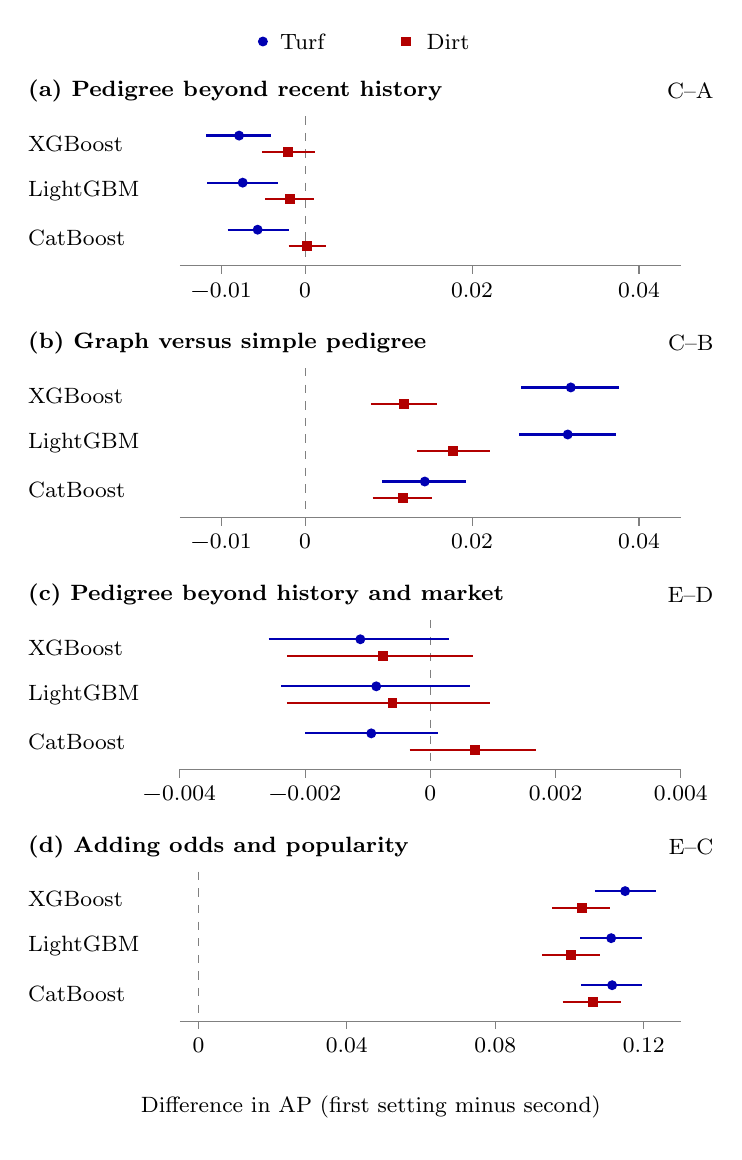
\begin{tikzpicture}[x=1pt,y=1pt,every node/.style={font=\footnotesize,inner sep=0pt}]
\useasboundingbox (0,-376) rectangle (248,23);
\fill[blue!70!black] (85,18) circle (1.8pt);
\node[anchor=west] at (91,18) {Turf};
\fill[red!70!black] (135,16.2) rectangle (138.6,19.8);
\node[anchor=west] at (144,18) {Dirt};
\node[anchor=west,font=\footnotesize\bfseries] at (0,0) {(a) Pedigree beyond recent history};
\node[anchor=east] at (248,0) {C--A};
\draw[gray,dashed] (100.25000,-9) -- (100.25000,-63);
\node[anchor=west] at (0,-19.0) {XGBoost};
\draw[blue!70!black,line width=0.8pt] (64.51879,-16) -- (88.08954,-16);
\fill[blue!70!black] (76.39434,-16) circle (1.8pt);
\draw[red!70!black,line width=0.8pt] (84.64982,-22) -- (103.72371,-22);
\fill[red!70!black] (92.28964,-23.8) rectangle (95.88964,-20.2);
\node[anchor=west] at (0,-36.0) {LightGBM};
\draw[blue!70!black,line width=0.8pt] (64.96685,-33) -- (90.31166,-33);
\fill[blue!70!black] (77.69231,-33) circle (1.8pt);
\draw[red!70!black,line width=0.8pt] (85.85195,-39) -- (103.52991,-39);
\fill[red!70!black] (93.03398,-40.8) rectangle (96.63398,-37.2);
\node[anchor=west] at (0,-53.0) {CatBoost};
\draw[blue!70!black,line width=0.8pt] (72.26109,-50) -- (94.30283,-50);
\fill[blue!70!black] (83.09692,-50) circle (1.8pt);
\draw[red!70!black,line width=0.8pt] (94.30643,-56) -- (107.76023,-56);
\fill[red!70!black] (99.19380,-57.8) rectangle (102.79380,-54.2);
\draw[gray] (55,-63) -- (236,-63);
\draw[gray] (70.08333,-63) -- (70.08333,-66);
\node[anchor=north] at (70.08333,-69) {\textminus{}0.01};
\draw[gray] (100.25000,-63) -- (100.25000,-66);
\node[anchor=north] at (100.25000,-69) {0};
\draw[gray] (160.58333,-63) -- (160.58333,-66);
\node[anchor=north] at (160.58333,-69) {0.02};
\draw[gray] (220.91667,-63) -- (220.91667,-66);
\node[anchor=north] at (220.91667,-69) {0.04};
\node[anchor=west,font=\footnotesize\bfseries] at (0,-91) {(b) Graph versus simple pedigree};
\node[anchor=east] at (248,-91) {C--B};
\draw[gray,dashed] (100.25000,-100) -- (100.25000,-154);
\node[anchor=west] at (0,-110.0) {XGBoost};
\draw[blue!70!black,line width=0.8pt] (178.40832,-107) -- (213.83245,-107);
\fill[blue!70!black] (196.25532,-107) circle (1.8pt);
\draw[red!70!black,line width=0.8pt] (124.01340,-113) -- (147.95615,-113);
\fill[red!70!black] (134.19110,-114.8) rectangle (137.79110,-111.2);
\node[anchor=west] at (0,-127.0) {LightGBM};
\draw[blue!70!black,line width=0.8pt] (177.59525,-124) -- (212.46516,-124);
\fill[blue!70!black] (195.14491,-124) circle (1.8pt);
\draw[red!70!black,line width=0.8pt] (140.74645,-130) -- (166.89437,-130);
\fill[red!70!black] (151.95101,-131.8) rectangle (155.55101,-128.2);
\node[anchor=west] at (0,-144.0) {CatBoost};
\draw[blue!70!black,line width=0.8pt] (128.06113,-141) -- (158.35925,-141);
\fill[blue!70!black] (143.49464,-141) circle (1.8pt);
\draw[red!70!black,line width=0.8pt] (124.62271,-147) -- (146.03829,-147);
\fill[red!70!black] (133.80366,-148.8) rectangle (137.40366,-145.2);
\draw[gray] (55,-154) -- (236,-154);
\draw[gray] (70.08333,-154) -- (70.08333,-157);
\node[anchor=north] at (70.08333,-160) {\textminus{}0.01};
\draw[gray] (100.25000,-154) -- (100.25000,-157);
\node[anchor=north] at (100.25000,-160) {0};
\draw[gray] (160.58333,-154) -- (160.58333,-157);
\node[anchor=north] at (160.58333,-160) {0.02};
\draw[gray] (220.91667,-154) -- (220.91667,-157);
\node[anchor=north] at (220.91667,-160) {0.04};
\node[anchor=west,font=\footnotesize\bfseries] at (0,-182) {(c) Pedigree beyond history and market};
\node[anchor=east] at (248,-182) {E--D};
\draw[gray,dashed] (145.50000,-191) -- (145.50000,-245);
\node[anchor=west] at (0,-201.0) {XGBoost};
\draw[blue!70!black,line width=0.8pt] (87.03301,-198) -- (152.25539,-198);
\fill[blue!70!black] (120.20592,-198) circle (1.8pt);
\draw[red!70!black,line width=0.8pt] (93.71246,-204) -- (160.80955,-204);
\fill[red!70!black] (126.46760,-205.8) rectangle (130.06760,-202.2);
\node[anchor=west] at (0,-218.0) {LightGBM};
\draw[blue!70!black,line width=0.8pt] (91.60293,-215) -- (159.96085,-215);
\fill[blue!70!black] (125.96019,-215) circle (1.8pt);
\draw[red!70!black,line width=0.8pt] (93.69963,-221) -- (167.05269,-221);
\fill[red!70!black] (130.02503,-222.8) rectangle (133.62503,-219.2);
\node[anchor=west] at (0,-235.0) {CatBoost};
\draw[blue!70!black,line width=0.8pt] (100.28261,-232) -- (148.36689,-232);
\fill[blue!70!black] (124.15522,-232) circle (1.8pt);
\draw[red!70!black,line width=0.8pt] (138.00584,-238) -- (183.73966,-238);
\fill[red!70!black] (159.73706,-239.8) rectangle (163.33706,-236.2);
\draw[gray] (55,-245) -- (236,-245);
\draw[gray] (55.00000,-245) -- (55.00000,-248);
\node[anchor=north] at (55.00000,-251) {\textminus{}0.004};
\draw[gray] (100.25000,-245) -- (100.25000,-248);
\node[anchor=north] at (100.25000,-251) {\textminus{}0.002};
\draw[gray] (145.50000,-245) -- (145.50000,-248);
\node[anchor=north] at (145.50000,-251) {0};
\draw[gray] (190.75000,-245) -- (190.75000,-248);
\node[anchor=north] at (190.75000,-251) {0.002};
\draw[gray] (236.00000,-245) -- (236.00000,-248);
\node[anchor=north] at (236.00000,-251) {0.004};
\node[anchor=west,font=\footnotesize\bfseries] at (0,-273) {(d) Adding odds and popularity};
\node[anchor=east] at (248,-273) {E--C};
\draw[gray,dashed] (61.70370,-282) -- (61.70370,-336);
\node[anchor=west] at (0,-292.0) {XGBoost};
\draw[blue!70!black,line width=0.8pt] (204.98782,-289) -- (227.01629,-289);
\fill[blue!70!black] (215.88242,-289) circle (1.8pt);
\draw[red!70!black,line width=0.8pt] (189.56320,-295) -- (210.43406,-295);
\fill[red!70!black] (198.48559,-296.8) rectangle (202.08559,-293.2);
\node[anchor=west] at (0,-309.0) {LightGBM};
\draw[blue!70!black,line width=0.8pt] (199.64401,-306) -- (221.82729,-306);
\fill[blue!70!black] (210.84720,-306) circle (1.8pt);
\draw[red!70!black,line width=0.8pt] (185.94791,-312) -- (206.65524,-312);
\fill[red!70!black] (194.53162,-313.8) rectangle (198.13162,-310.2);
\node[anchor=west] at (0,-326.0) {CatBoost};
\draw[blue!70!black,line width=0.8pt] (200.02759,-323) -- (222.14920,-323);
\fill[blue!70!black] (211.18912,-323) circle (1.8pt);
\draw[red!70!black,line width=0.8pt] (193.31513,-329) -- (214.43024,-329);
\fill[red!70!black] (202.58211,-330.8) rectangle (206.18211,-327.2);
\draw[gray] (55,-336) -- (236,-336);
\draw[gray] (61.70370,-336) -- (61.70370,-339);
\node[anchor=north] at (61.70370,-342) {0};
\draw[gray] (115.33333,-336) -- (115.33333,-339);
\node[anchor=north] at (115.33333,-342) {0.04};
\draw[gray] (168.96296,-336) -- (168.96296,-339);
\node[anchor=north] at (168.96296,-342) {0.08};
\draw[gray] (222.59259,-336) -- (222.59259,-339);
\node[anchor=north] at (222.59259,-342) {0.12};
\node at (124,-367) {Difference in AP (first setting minus second)};
\end{tikzpicture}

\caption{Historical AP contrasts. Positive values favor the first setting. Points average paired seed differences; bars are descriptive 95\% whole-race bootstrap intervals, conditional on fitted models and unadjusted for multiplicity. Panels (a)--(b) share a scale; others differ. Market fields are retrospective and absent from the new arms.}
\label{fig:historical_contrasts}
\end{figure}

\subsection{Historical Market and Parent-ID Context}
\begin{table*}[!t]
\caption{Historical Market-Information Scores Across All Families and Surfaces}
\label{tab:historical_market}
\centering
\begin{tabular}{llrrrrrr}
\hline
& & \multicolumn{3}{c}{Entry AP} & \multicolumn{3}{c}{Mean Hit@3} \\
Family & Surface & D & E & F & D & E & F \\
\hline
XGBoost & Turf & 0.5792 & 0.5781 & 0.5679 & 0.5400 & 0.5382 & 0.5363 \\
XGBoost & Dirt & 0.5582 & 0.5574 & 0.5507 & 0.5285 & 0.5287 & 0.5261 \\
LightGBM & Turf & 0.5784 & 0.5775 & 0.5668 & 0.5387 & 0.5386 & 0.5360 \\
LightGBM & Dirt & 0.5577 & 0.5571 & 0.5496 & 0.5291 & 0.5283 & 0.5269 \\
CatBoost & Turf & 0.5793 & 0.5783 & 0.5676 & 0.5395 & 0.5380 & 0.5365 \\
CatBoost & Dirt & 0.5582 & 0.5589 & 0.5511 & 0.5286 & 0.5275 & 0.5265 \\
\hline
\end{tabular}
\par\smallskip Historical three-seed means: D adds final odds and popularity to history; E adds them to the original graph pipeline; F uses final odds alone. The market fields are retrospective and are not inputs in the new four-arm study.
\end{table*}

Table~\ref{tab:historical_market} retains every family and surface for the earlier market-informed settings; Fig.~\ref{fig:historical_contrasts} retains all four historical AP contrasts. Odds alone gives AP 0.5668--0.5679 on turf and 0.5496--0.5511 on dirt. In the historical E--D comparison, all six AP intervals include zero. Adding final odds and popularity to C (E--C) increases AP by approximately 0.1004--0.1150 and Hit@3 by 0.066--0.078. These are independently tuned comparisons with retrospective final-market inputs, not isolated causal effects or evidence of betting profit. They do not test the new $G_{\mathrm{ancestor}}$ or P arms with market features.





Historically, C outperformed the tested categorical-parent B pipeline, but B was weaker than A; this does not establish added value beyond history or superiority over the supervised P comparator. Test sire/dam identifiers were unseen in the historical training-surface vocabulary for 30.04\%/38.73\% of turf entries and 28.75\%/42.15\% of dirt entries. The earlier no-observed-history subgroup was added after test release and is not necessarily a true debut cohort. The corrected deterministic random baseline has Hit@3 of 0.2431 turf and 0.2161 dirt, against analytical expectations 0.2433 and 0.2188.

\subsection{Interpretation and Limitations}
The contrasts concern the specified independently tuned pipelines and their feature groups. They do not measure a causal effect of pedigree, isolate fallback from all other representation differences, or establish whether a different graph architecture or ancestry model would help. A common ancestor construction rule does not equate coverage or distributions across partitions. The graph retains the influence of focal horses and later training roots; retrospective pedigree collection does not establish historical record availability. P is a simple supervised comparator with left-censored source history and an increasingly aged frozen map. Its results do not describe an always-updated parent model.

The previously examined test set, unadjusted multiple comparisons and dependence from repeated horses limit inference. Three paired seeds confound graph and classifier randomness; the race bootstrap is conditional on the fitted seeds. The observed collection omits some histories and does not cover all racing jurisdictions. Race-day variables may not have been available at a common prediction horizon, and no dedicated ranker, prospective deployment or betting-profit evaluation is included. These limits constrain transfer and operational claims even if a contrast is favorable.

\section{Conclusion}
In this exploratory same-cohort evaluation, the tested ancestor-rule graph pipeline did not consistently improve AP beyond either recent history or the specified chronological parent-performance pipeline. Turf primary contrasts were negative; dirt intervals included zero. The secondary CatBoost dirt comparison favored the ancestor-rule pipeline over the original mixed pipeline, but does not identify a fallback effect or establish improvement over the primary controls. Historical retrospective market comparisons remain separate and do not evaluate the new four arms beyond market information. Future work requires historically timestamped inputs and an unexamined cohort.

\section*{Data and Code Availability}
Race and pedigree records came from Netkeiba \cite{netkeibaRace,netkeibaDb}. Public data, graph/feature exports, models and predictions are on Kaggle (version 1): \url{https://www.kaggle.com/datasets/charischerw/jra-pedigree-graph-study-2010-2025}. Code, configurations, aggregate results and reproduction instructions are at \url{https://github.com/CharisBerlian/jra-pedigree-graph-study} (release v1.0.5-paper). Data/results use CC BY 4.0; study-authored code uses MIT, with third-party licenses retained. The repository documents environments and limits; independent full-data retraining has not been established.

% Keep the reference heading and entries together after the pending wide figure.
\newpage
\IEEEtriggeratref{11}
\begin{thebibliography}{00}

\bibitem{jraResults}
Japan Racing Association, ``JRA race card and results.'' [Online]. Available: \url{https://jra.jp/JRAEN/AP/common/main}. Accessed: Apr. 30, 2026.

\bibitem{netkeibaRace}
Netkeiba, ``Race results (race.netkeiba.com).'' [Online]. Available: \url{https://race.netkeiba.com/}. Accessed: Sept.~9, 2026.

\bibitem{netkeibaDb}
Netkeiba, ``Pedigree database (db.netkeiba.com).'' [Online]. Available: \url{https://db.netkeiba.com/}. Accessed: Sept.~9, 2026.

\bibitem{grover2016}
A. Grover and J. Leskovec, ``Node2vec: Scalable feature learning for networks,'' in \emph{Proc. 22nd ACM SIGKDD Int. Conf. Knowledge Discovery and Data Mining (KDD)}, 2016, pp. 855--864, doi: \url{10.1145/2939672.2939754}.

\bibitem{silverman2013}
N. Silverman and M. Suchard, ``Predicting horse race winners through a regularized conditional logistic regression with frailty,'' \emph{The Journal of Prediction Markets}, vol. 7, no. 1, pp. 43--52, 2013, doi: \url{10.5750/jpm.v7i1.595}.

\bibitem{pudaruth2013}
S. Pudaruth, N. Medard, and Z. B. Dookhun, ``Horse racing prediction at the Champ De Mars using a weighted probabilistic approach,'' \emph{International Journal of Computer Applications}, vol. 72, no. 5, pp. 39--42, 2013, doi: \url{10.5120/12493-9048}.

\bibitem{bailey2022}
E. Bailey, J. L. Petersen, and T. S. Kalbfleisch, ``Genetics of Thoroughbred racehorse performance,'' \emph{Annual Review of Animal Biosciences}, vol. 10, pp. 131--150, 2022, doi: \url{10.1146/annurev-animal-020420-035235}.

\bibitem{oda2024}
D. Oda and A. Onogi, ``Assessing the predictability of racing performance of Thoroughbreds using mixed-effects model,'' \emph{Journal of Animal Breeding and Genetics}, vol. 141, no. 1, pp. 24--32, 2024, doi: \url{10.1111/jbg.12822}.

\bibitem{gulum2018}
M. A. Gulum, ``Horse racing prediction using graph-based features,'' M.S. thesis, Univ. Louisville, 2018, doi: \url{10.18297/etd/2953}.

\bibitem{oikawa2024}
{\japanesefont 及川颯希} and {\japanesefont 田村篤史},\newline ``{\japanesefont 血統情報を用いたGNNによる競走馬の成績予測}'' [Predicting racehorse performance using graph neural networks based on pedigree information], IPSJ Technical Report, vol. 2024-IS-170, no. 7, pp. 1--6, 2024. [Online]. Available: \url{https://jglobal.jst.go.jp/detail?JGLOBAL_ID=202502212071299786}.

\bibitem{sugiura2026}
S. Sugiura, ``Leakage-aware pre-event machine learning evaluation for horse-race prediction under temporal validation,'' \emph{Frontiers in Artificial Intelligence}, vol. 9, Art. no. 1896192, 2026, doi: \url{10.3389/frai.2026.1896192}.

\bibitem{chung2024}
J. Chung, D. Shin, S. Hwang, and G. Park, ``Horse race rank prediction using learning-to-rank approaches,'' \emph{The Korean Journal of Applied Statistics}, vol. 37, no. 2, pp. 239--253, 2024, doi: \url{10.5351/KJAS.2024.37.2.239}.

\bibitem{jraStats2yo}
Japan Racing Association, ``Number of runners according to age and breed (1990--): 2-y-o Thoroughbreds,'' \emph{Racing Statistics 2025}. [Online]. Available: \url{https://japanracing.jp/_statistics/2025/s02.html}. Accessed: Aug. 16, 2026.

\bibitem{jraStats3up}
Japan Racing Association, ``Number of runners according to age and breed (1990--): 3-y-o \& up Thoroughbreds,'' \emph{Racing Statistics 2025}. [Online]. Available: \url{https://japanracing.jp/_statistics/2025/s03.html}. Accessed: Aug. 16, 2026.

\bibitem{chen2016}
T. Chen and C. Guestrin, ``XGBoost: A scalable tree boosting system,'' in \emph{Proc. 22nd ACM SIGKDD Int. Conf. Knowledge Discovery and Data Mining (KDD)}, 2016, pp. 785--794, doi: \url{10.1145/2939672.2939785}.

\bibitem{ke2017}
G. Ke, Q. Meng, T. Finley, T. Wang, W. Chen, W. Ma, Q. Ye, and T.-Y. Liu, ``LightGBM: A highly efficient gradient boosting decision tree,'' in \emph{Advances in Neural Information Processing Systems 30}, 2017, pp. 3149--3157.

\bibitem{prokhorenkova2018}
L. Prokhorenkova, G. Gusev, A. Vorobev, A. V. Dorogush, and A. Gulin, ``CatBoost: Unbiased boosting with categorical features,'' in \emph{Advances in Neural Information Processing Systems 31}, 2018, pp. 6638--6648.

\bibitem{saito2015}
T. Saito and M. Rehmsmeier, ``The precision-recall plot is more informative than the ROC plot when evaluating binary classifiers on imbalanced datasets,'' \emph{PLOS ONE}, vol. 10, no. 3, Art. no. e0118432, 2015, doi: \url{10.1371/journal.pone.0118432}.

\end{thebibliography}

\end{document}
